\documentclass{article}

\usepackage[top=1in,left=1.5in,right=1.5in,bottom=1.5in]{geometry}

\usepackage{pgfplots}
\usetikzlibrary{angles, arrows.meta, calc, quotes}
\pgfplotsset{width=0.8\textwidth,compat=1.18}

\usepackage{subcaption}

\usepackage{booktabs}

\usepackage{graphicx}
\let\rfb\reflectbox
\graphicspath{ {images} }

\usepackage{cancel}

\usepackage{mathtools}

\usepackage{nicefrac}
\newcommand{\flippedfrac}[2]{\rfb{\nicefrac{\rfb{#2}}{\rfb{#1}}}}



\usepackage{amsthm}
\renewcommand{\qedsymbol}{$\blacksquare$}
\usepackage{amssymb}
\usepackage{amsmath}
\newcommand\numberthis{\addtocounter{equation}{1}\tag{\theequation}}
\DeclareMathOperator*{\argmax}{arg\,max}
\DeclareMathOperator*{\argmin}{arg\,min}

\usepackage{hyperref}
\hypersetup{
    colorlinks = true,
}


\usepackage{titling}
\title{Exercise Set 4 - Reinforcement Learning}
\newcommand{\subtitle}[1]{%
  \posttitle{%
    \par\end{center}
    \begin{center}\large#1\end{center}
    \vskip0.5em}%
}
\makeatother
\subtitle{Control with approximation and policy gradients}
\author{Giulio Starace - 13010840}
\date{\today}

\begin{document}
\maketitle
\section*{Homework: Geometry of linear value-function approximation (Application)}
\begin{enumerate}
	\item \label{q:7.4.1} To compute the Bellman error vector after initialization, we compute the
	      Bellman error for each state. We first recall the definition of the Bellman operator $B^\pi$:
	      \begin{equation}
		      (B^\pi v)(s) ~ \dot{=} ~ \sum_a \pi(a | s) \sum_{s', r} p(s', r | s, a) \left[ r + \gamma
			      v(s') \right].
	      \end{equation}
	      We can plug this into the definition of the Bellman error:
	      \begin{align*}
		      \overline{\delta}_w(s) & = B^\pi v_w - v_w                                       \\
		                             & = \sum_a \pi(a | s) \sum_{s', r} p(s', r | s, a) \left[
			      r + \gamma v_w(s') \right] - v_w(s).
	      \end{align*}
	      For $s_0$, we have a single action available that is always taken, so our $\sum_a
		      \pi(a | s)$ term disappears and we are left with:
	      \begin{equation}
		      \overline{\delta}_w(s) = \sum_{s', r} p(s', r | s) \left[r + \gamma
			      v_w(s') \right] - v_w(s)
	      \end{equation}
	      Our action always leads to the same state, with the same reward (of 0), so we can simplify further
	      and write
	      \begin{equation}
		      \overline{\delta}_w(s) = \gamma v_w(s') - v_w(s).
	      \end{equation}
	      Finally, we have that $v_{w, s} = w \cdot \phi_s$, so that we can write
	      \begin{equation}
		      \overline{\delta}_w(s) = \gamma w \cdot \phi_{s'} - w \cdot \phi_s.
	      \end{equation}
	      The same arguments can be applied to $s_1$, so we can write the Bellman error
	      \textit{vector} as
	      \begin{equation}
		      \text{BE}(w) = \left(\overline{\delta}_w(s_0), ~ \overline{\delta}_w(s_1) \right)^T = \left(
		      \gamma w \cdot \phi_{s_1} - w \cdot \phi_{s_0}, ~ \gamma w \cdot \phi_{s_0} - w
		      \cdot \phi_{s_1} \right)^T.
	      \end{equation}
	      We can plug in our values $w =1$, $\phi_{s_0} = 2$, $\phi_{s_1} = 1$, and $\gamma =1$ and
	      obtain
	      \begin{equation}
		      \text{BE}(w) = \left(1 \cdot1 - 1 \cdot 2, ~ 1 \cdot 2 - 1 \cdot 1\right)^T = \left(-1, ~ 1\right)^T.
	      \end{equation}
	\item The Mean Squared Bellman Error $\overline{\text{BE}}(w)$ is the measure of the overall error in the
	      value function, computed by taking the $\mu$ weighted norm of the Bellman error vector. Here,
	      $\mu$ is a distribution $\mu : \mathcal{S} \rightarrow \left[0, 1\right]$ specifying the extent
	      to which each state is considered in the computation. Mathematically:
	      \begin{equation}
		      \overline{\text{BE}}(w) = \lVert \text{BE}(w) \rVert^2_\mu = \sum_s \mu(s) \overline{\delta}_w(s)^2.
	      \end{equation}
	      In our case, this would be expressed as
	      \begin{equation}
		      \overline{\text{BE}}(w) = \mu(s_0) \cdot (-1)^2 + \mu(s_1) \cdot 1^2 = \mu(s_0) + \mu(s_1)
		      = \sum_s \mu(s).
	      \end{equation}
	\item The target values $B^\pi v_w$ we found in question \ref{q:7.4.1}. are 1 for $s_0$ and 2 for
	      $s_1$. The $w$ that results in the value function that is closest can be applied using
	      a least-squares regression:
	      \begin{align*}
		      \beta & = \argmin_\beta  \lVert \mathbf{Y} - w \mathbf{X} \rVert^2               \\
		      w     & = \argmin_w  \lVert (1, ~2 )^T - w (\phi_{s_0}, ~ \phi_{s_1})^T \rVert^2 \\
		            & = \argmin_w\lVert (1, ~2 )^T - w (2, 1)^T \rVert^2. \numberthis
	      \end{align*}
	      This has a closed-form solution:
	      \begin{equation}
		      \beta = \left(\mathbf{X}^T \mathbf{X}\right)^{-1} \mathbf{X}^T \mathbf{Y},
	      \end{equation}
	      which for our numbers gives $w = 4/5$.
	\item The plot of $v_w$, $B^\pi v_w$ and $\Pi B^\pi v_w$ is shown in Figure \ref{fig:7.4.4}. TODO
	      % put image here		
	      \begin{figure}[ht!]
		      \centering
		      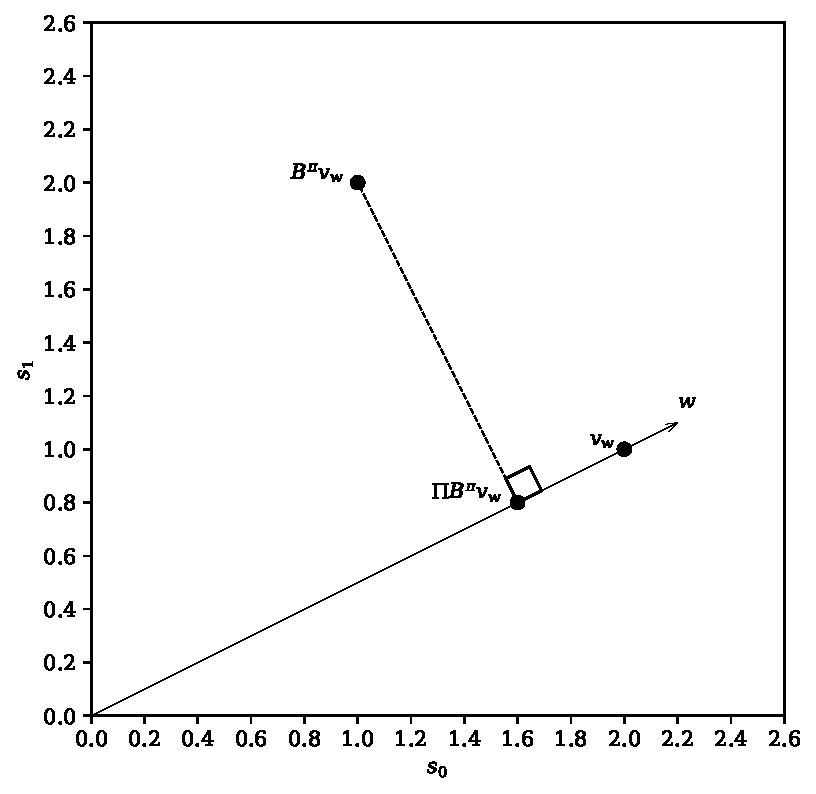
\includegraphics[width=0.6\textwidth]{images/7.4.4.pdf}
		      \caption{TODO}
		      \label{fig:7.4.4}
	      \end{figure}

\end{enumerate}
\section*{Homework: Coding Assignment - Deep Q Networks}
\begin{enumerate}
	\item Coding answers have been submitted on codegra under the group ``stalwart cocky sawly".
	\item hello world
\end{enumerate}

\section*{Homework: REINFORCE}
\begin{enumerate}
	\item \begin{enumerate}
		      \item \label{8.4.1a} The update to the policy parameter  $\theta$ under classical
		            REINFORCE after the $e$th episode is given by
		            \begin{equation}\label{eq:policy_update}
			            \theta_{e+1} \leftarrow \theta_e + \alpha \widehat{\nabla_\theta J},
		            \end{equation}
		            where $\widehat{\nabla J}$ is an estimate of the gradient the expectation of the
		            return $G(\tau_e)$ for a given trajectory $\tau$, and $\alpha$ is the learning rate.
		            This is given by
		            \begin{equation}
			            \widehat{\nabla_\theta J} = \frac{1}{N} \sum^N_{i=1}\left[G(\tau_i)
				            \sum_{t=0}^T\nabla_\theta \log \pi_\theta (a_t^i | s_t^i)\right],
		            \end{equation}
		            where $N$ is the number of trajectories observed, and $\pi_\theta$ is the policy we
		            are parametrising with $\theta$. Because we are interested in the update
		            per-episode, $N=1$ and our equation simplifies to
		            \begin{equation}\label{eq:reinforce_episode_grad}
			            \widehat{\nabla_\theta J} = G(\tau_e) \sum_{t=0}^T\nabla_\theta \log \pi_\theta (a_t^i
			            | s_t^i)
		            \end{equation}
		            Because in our case $\theta$ is split into $\theta_a$ and $\theta_b$, where an
		            action in state $A$ only depends on $\theta_a$ and the action in state $B$ only
		            depends on $\theta_b$, we can treat the update to each parameter separately,
		            obtaining
		            \begin{align}
			            \theta^{e+1}_a & \leftarrow \theta^e_a + \alpha \widehat{\nabla_{\theta_a} J}  \\
			            \theta^{e+1}_b & \leftarrow \theta^e_b + \alpha \widehat{\nabla_{\theta_b} J}.
		            \end{align}
		            $\widehat{\nabla_{\theta_{a/b}}J}$ takes the same form as
		            (\ref{eq:reinforce_episode_grad}), but now only depends on the actions taken in
		            state $A$ or $B$ respectively. This leaves us with
		            \begin{align}
			            \widehat{\nabla_{\theta_a} J} & = G(\tau_e) \sum_{t : s_t = A}^T\nabla_{\theta_a}
			            \log \pi_\theta(a_t^i| A, \theta_a)                                               \\
			            \widehat{\nabla_{\theta_b} J} & = G(\tau_e) \sum_{t : s_t = B}^T\nabla_{\theta_b}
			            \log \pi_\theta(a_t^i| B, \theta_b)
		            \end{align}
		            We can plug this into our updates for each part of $\theta$ and obtain
		            \begin{align}
			            \theta^{e+1}_a & \leftarrow \theta^e_a + \alpha G(\tau_e) \sum_{t : s_t
				            = A}^T\nabla_{\theta_a} \log \pi_\theta(a_t^i| A, \theta_a)
			            \label{eq:reinforce_a_update}                                           \\
			            \theta^{e+1}_b & \leftarrow \theta^e_b + \alpha G(\tau_e) \sum_{t : s_t
				            = B}^T\nabla_{\theta_b} \log \pi_\theta(a_t^i| B,
			            \theta_b),\label{eq:reinforce_b_update}
		            \end{align}
		            where the trajectory $\tau_e$ will be different for each episode $e$. We can plug in the
		            values given from our sampled episodes and obtain the following four updates:
		            \begin{align}
			            \theta^1_a & \leftarrow \theta^0_a + \alpha \cdot 175 \cdot
			            \nabla_{\theta_a}\left[ \log \pi_\theta(1| A, \theta_a) + \log \pi_\theta(2|
			            A, \theta_a)\right]                                         \\
			            \theta^2_a & \leftarrow \theta^1_a - \alpha \cdot 60 \cdot
			            \nabla_{\theta_a}\left[ \log \pi_\theta(1| A, \theta_a) + \log \pi_\theta(2|
			            A, \theta_a)\right]                                         \\
			            \theta^1_b & \leftarrow \theta^0_b + \alpha \cdot 175 \cdot
			            \nabla_{\theta_b}\left[ \log \pi_\theta(2| B, \theta_b) + \log \pi_\theta(2|
			            B, \theta_b)\right]                                         \\
			            \theta^1_b & \leftarrow \theta^0_b - \alpha \cdot 60 \cdot
			            \nabla_{\theta_b}\left[ \log \pi_\theta(1| B, \theta_b) + \log \pi_\theta(1|
				            B, \theta_b)\right]
		            \end{align}
		      \item When using REINFORCE/G(MO)MDP, we now have a different general estimate of the
		            gradient of the expectation of the return, $\widehat{\nabla J},$ given by
		            \begin{equation}
			            \widehat{\nabla_\theta J} = \frac{1}{N} \sum^N_{i=1}\left(\sum_{t=1}^T r_t
			            \sum_{t'=1}^t\nabla_\theta \log \pi_\theta (a_{t'} | s_{t'})\right),
		            \end{equation}
		            where $r_t$ is the reward at time $t$ for episode $i$. We can apply the same
		            reasoning used in \ref{8.4.1a} and obtain the update rule per episode for each
		            split of $\theta$:
		            \begin{align}
			            \theta^{e+1}_a & \leftarrow \theta^e_a + \alpha \sum_{t=1}^T r_t \sum_{t' \in
			            \left\{z:s_{z} = A \land z \leq t\right\}}  \nabla_{\theta_a} \log \pi_\theta
			            (a_{t'} | A, \theta_a)\label{eq:gpomdp_a_update}                              \\
			            \theta^{e+1}_b & \leftarrow \theta^e_b + \alpha \sum_{t=1}^T r_t \sum_{t' \in
			            \left\{z:s_{z} = B \land z \leq t\right\}}\nabla_{\theta_b} \log \pi_\theta
			            (a_{t'} | B, \theta_b)\label{eq:gpomdp_b_update}
		            \end{align}
		            where the rewards $r_t$ will be different depending on the episode. We can plug in the
		            values given from our sampled episodes and obtain the following four updates:
		            \begin{align}
			            \theta^1_a & \leftarrow \theta^0_a + \alpha \cdot \nabla_{\theta_a} \bigl[175
			            \cdot \log \pi (1 | A, \theta_a) - 25 \cdot \log \pi (2 | A, \theta_a)  \bigr]   \\
			            \theta^2_a & \leftarrow \theta^1_a + \alpha \cdot \nabla_{\theta_a} \bigl[-
			            60 \cdot \log \pi (1 | A, \theta_a) + 40 \cdot \log \pi (2 | A, \theta_a) \bigr] \\
			            \theta^1_b & \leftarrow \theta^0_b + \alpha \cdot \nabla_{\theta_b}
			            \bigl[-8 \cdot \log \pi (2 | B, \theta_B) \bigr]                                 \\
			            \theta^2_b & \leftarrow \theta^1_b + \alpha \cdot \nabla_{\theta_b}
			            \bigl[30 \cdot \log \pi (1 | B, \theta_B) \bigr]
		            \end{align}
	      \end{enumerate}
	\item hello world
	\item hello world
	\item hello world
	\item hello world
\end{enumerate}


\end{document}

